\documentclass[jou,apacite]{apa6}
\usepackage{amsmath}
\usepackage{amsfonts} 
\usepackage{graphicx}
\usepackage{subcaption}

\title{Reducing Global Cumulative Odometry Error with Overhead Camera Localization in the Soar Cognitive Architecture}
\author{Minxing Pan and Nicholas C. Matton}
\affiliation{The University of Michigan}
\shorttitle{Overhead Camera Localization}

\abstract{ Abstract, todo }
\keywords{robot mapping, localization, linear algebra, computer vision}

\rightheader{Overhead Camera Localization}
\leftheader{Pan and Matton}

\begin{document}
\maketitle

\section{Introduction}
Intelligent robots need a navigation map of their surroundings in order to efficiently travel and complete tasks in their local environment. In simulations, the exact location of a robot is usually consistent with that of the robot’s own navigation maps. Physical robots, however, can introduce odometry error into the mapping process. Odometry is calculating relative position based on the measurements of sensorimotor data. While odometry provides easily accessible real-time robot pose, its accuracy is dependent on if the wheel revolutions measured by the encoders can be fully translated into linear displacement relative to the ground \cite{Borenstein}.

For our project, Anki’s Cozmo robots are used to present a method of correcting odometry error in mobile robots. Cozmo is a fist-sized robot capable of exploring unknown environments and interacting with cubes. It builds a two-dimensional navigation memory map (nav map) of its surroundings as it travels. The nav map is built mostly based on where Cozmo’s camera picks up the objects and where Cozmo detects drops and visible edges. Unlike standard occupancy maps, which only compute the probability of a grid space being occupied by an object, the nav map also annotates the type of object in the occupancy grid. The nav map is stored as a quad-tree, in which leaf nodes hold the contents such as cubes and chargers, and all other nodes split into four children. Child node indices are stored in the x, y orientation shown in figure \ref{fig:navmap} \cite{Anki}.

\begin{figure}
	\begin{center}
		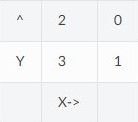
\includegraphics[scale=1]{navmap.jpg}
	\end{center}
	\caption{A node in the navmap.
		Leaf nodes contain content, all other nodes are split into 4 equally sized children. Child node indices are stored in the following X,Y orientation:}
	\label{fig:navmap}
\end{figure}

In addition to the nav map, Cozmo relies on odometry to estimate its position and rotation (Cozmo pose) as it travels. Cozmo uses a right-handed coordinate system, in which the y-axis is to the left of the x-axis, and counterclockwise rotation is considered positive. When first initialized, Cozmo recognizes its current pose as the Cozmo origin, such that its x, y, z, rotation, pitch, and yaw are all zeros, and the direction it faces towards is the positive x axis. 

In Cozmo odometry, the perceived travel distance is based on the encoder values of the motors, and the actual travel distance is the displacement of Cozmo relative its previous position. Some of the systematic odometry errors include “unequal wheel diameters” and the “misalignment of wheels” \cite{Borenstein}. Because Cozmo drives with treads, the horizontal instability of the treads while driving contributes to the misalignment. The wear and tear of tread on either side causes unequal diameters. Consequently, the Cozmo odometry can be inaccurate. For example, when Cozmo turns, Cozmo’s perceived sensorimotor data can be a few degrees different from the actual travel data. This cumulation in odometry drift causes the Cozmo origin to deviate, leading to an inconsistent perceived robot pose with regards to the actual robot pose. The cumulative odometry error causes problems in robot exploration and navigation over time.

Our project runs programs controlling the Cozmo robots on the Soar Cognitive Architecture. “Soar is a general cognitive architecture that integrates knowledge-intensive reasoning, reactive execution, hierarchical reasoning, planning, and learning from experience, with the goal of creating a general computational system that has the same cognitive abilities as humans” 
\cite{Laird}. Our program uses the Cozmo-Soar Interface to interact with the Cozmo robots. The Cozmo-Soar Interface is a python-based interface between Soar and Cozmo based on the Soar Markup Language (SML), PySoarLib, and the Cozmo SDK \cite{Mininger}. “The purpose of the interface is to allow a Soar agent to control a fully-embodied Cozmo robot, thereby embodying the Soar agent in the real world and enabling cognitive experiments to be run on a small, flexible, and robust platform” \cite{Boggs}. One of the research goals of CozmoSoar is interactive task learning, specifically training the Cozmo robots new tasks through natural language instruction. The movement and navigation in said programs require a global coordinate frame, but the Cozmo odometry error made it too inaccurate (Miniger, 2019). Therefore, we need to come up with a method to reduce the cumulative odometry error in Cozmo in a global coordinate frame.


\section{Method}
We are approaching the problem of inconsistent perceived robot pose and the actual robot pose with an overhead camera system that uses localization to correct the Cozmo's pose. The vision processing is done using OpenCV version 4.1.1. OpenCV is an open-source computer vision library. Other researchers have modeled odometry error using Simultaneous Localization and Mapping (SLAM) with advanced sonar systems \cite{Kleeman}. Another researcher implemented scale-invariant visual landmarks to correct local odometry while only using odometry to predict the region to search for landmarks \cite{se}. Both methods are effective but require more computing power, expensive equipment, longer processing time, and more complicated math models. Our method of overhead camera localization requires less computing power and inexpensive equipment, but can achieve similarly accurate results.

\subsection{Camera Calibration}
The Logitech HD Pro Webcam C920, Widescreen Video Calling and Recording, 1080p Camera, Desktop or Laptop Webcam is selected for our overhead camera system. Camera Calibration is necessary because each camera may introduce some distortion to the images it perceives. The two major types of distortion are radial distortion, which causes straight lines to appear curved, and tangential distortion, which causes some areas in the image to look nearer than actual \cite{OpenCV}. 

The OpenCV library provides a function to calculate the distortion coefficients needed to correct the images with a calibration process using a checkerboard image. In this project, a nine by six monochromatic checkerboard image provided by OpenCV was used to calibrate the camera. Our program collects a stack of 100 different images of the checkerboard at different angles and distances to the camera. Then our program uses the OpenCV function of calibrating the camera to calculate the distortion coefficients. 
After calibrating the camera once in the lab environment with ambient lighting, the calibration data can be used to undistort new images streamed by the camera prior to any further image processing.

\subsection{Pose Estimation}
Since cumulative odometry drift causes the Cozmo origin to deviate, there needs to be a reliable method to estimate the robot pose and recalibrate the Cozmo origin. Pose estimation can be done based on finding correspondences between objects in the real world and their two-dimensional image taken by the camera \cite{OpenCV}. While one could estimate robot pose with a multi-objective Convolutional Neural Network, that process requires hundreds of robot images for training \cite{Miseikis}.

In this project, binary square fiducial markers are selected, because an individual marker’s four corners provide enough correspondences to establish a pose relative to the camera. The Cozmo robot can be identified by an ArUco marker placed directly on top of it. An ArUco marker is a square marker with a distinguishable black border that allows for fast detection in an image and an inner binary matrix that encodes an identifier (Id) \cite{Garrido-Jurado}. Because only two to three identifying markers are needed, the smallest ArUco dictionary are selected for the fastest processing time. ArUco markers that are four bits by four bits markers with 200 pixels in each and one bit in the border are printed and cut out. One marker is taped directly on top of Cozmo while the camera is placed straight above the Cozmo exploration environment.

Our program can then estimate the robot pose with images streamed from the calibrated camera. The OpenCV algorithm can estimate the pose based on a single ArUco marker and the camera calibration data. For every image frame fed to the program, the function returns the rotation and translation vectors of each detected marker in the image. The two vectors transform a three-dimensional point of an object to a frame relative to the camera \cite{OpenCV}. The pose obtained from this method is of the marker in relation to the camera. Therefore, additional processing is needed to turn the pose into a right-handed world coordinate system that can be easily translated to and from the Cozmo coordinate system.

Another ArUco marker is then placed at the bottom left corner of the Cozmo exploration environment and set that as the origin of our world coordinates. Both the translation and rotation vector of the world origin are then subtracted from those of the robot pose marker. This way, the robot pose is no longer moving relative to the camera, but rather in relation to a fixed point in the Cozmo exploration environment. Furthermore, because the camera captures a mirrored image of the actual setup, the y-axis and the yaw need to be flipped to make the image consistent with the real world.

After the calculation of the translation and rotation vectors of the robot pose in relation to the world origin in a right-handed world coordinate system, the two vectors needs to be translated into x, y, z, roll, pitch, and yaw values. Conveniently, the translation vector’s three values are the x, y, and z values of the robot position coordinates that can be used without any other calculation. The rotation vector, however, requires additional computation to transform into euler angles (roll, pitch, and yaw). First, Rodrigues' Rotation Formula converts the rotation vector to a three by three rotation matrix. Then, an implementation similar to that of MATLAB is modified to convert the rotation matrix to euler angles \cite{Mallick}. Last but not least, the only rotation needed for our application is that with regards to the z-axis (yaw), so only the third value of the Euler angles is needed.


\subsection{Linear Transformations}
A method to acquire the real time robot pose in the world coordinate system has been established so far. Cozmo, however, has its own coordinate system described in the Introduction section. Our program can convert to and from the two coordinate systems.

\begin{figure}
	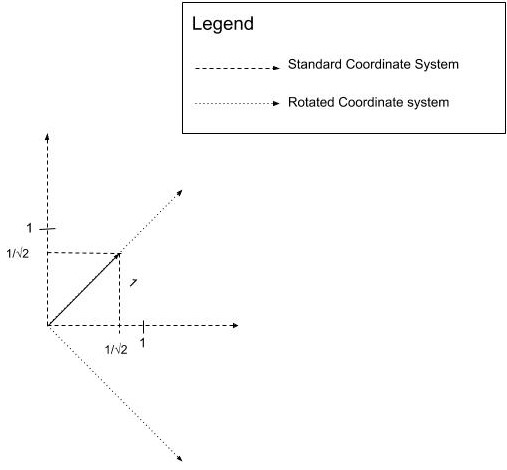
\includegraphics[width=\linewidth]{rotation_difference.jpg}
	\caption{The same vector represented by the coordinates [$\frac{1}{\sqrt2}$, $\frac{1}{\sqrt2}$] in the standard coordinate system is represented by the coordinates [0, 1] in a rotated coordinate system}
	\label{fig:rotdiff}
\end{figure}

There are two differences in the coordinate systems: rotation and translation. A rotational difference creates an inconsistency in bases between the two coordinate systems. For example, the same vector represented by the coordinates [$\frac{1}{\sqrt2}$, $\frac{1}{\sqrt2}$] in one coordinate system can be represented by the coordinates [0, 1] in another (see Figure \ref{fig:rotdiff}). Because the axes’ for both the Cozmo and the world coordinate systems are orthogonal, this implies that both coordinate systems have orthogonal bases \cite{Bretscher}
. Rotation matrices can therefore be used as change of basis matrices $S_{\mathfrak{C}\rightarrow\mathfrak{W}}$ and $S_{\mathfrak{W}\rightarrow\mathfrak{C}}$ to convert between the two bases (Equation \ref{eq:s}). $\mathfrak{C}$ is the Cozmo basis; $\mathfrak{W}$ is the world basis; r is the difference between the rotation $\theta_w$ of the world origin and the rotation $\theta_c$ of the Cozmo origin (Equation \ref{eq:r}).
\begin{equation} \label{eq:r}
r = \theta_w - \theta_c
\end{equation}
\begin{equation} \label{eq:s}
S_{\mathfrak{C}\rightarrow\mathfrak{W}}=
\begin{bmatrix}
cos(r) & sin(r) & 0 \\
-sin(r) & cos(r) & 0 \\
0 & 0 & 1
\end{bmatrix}
\end{equation}

$S_{\mathfrak{C}\rightarrow\mathfrak{W}}$ changes a vector from Cozmo's basis to the world's basis (Equation \ref{eq:cw}), while its inverse $S_{\mathfrak{W}\rightarrow\mathfrak{C}}$ changes a vector from the world's basis to Cozmo's basis (Equation \ref{eq:wc}).
\begin{equation} \label{eq:cw}
[V]_\mathfrak{W} = S_{\mathfrak{C}\rightarrow\mathfrak{W}} \cdot [V]_\mathfrak{C}
\end{equation}
\begin{equation} \label{eq:wc}
[V]_\mathfrak{C} = S_{\mathfrak{W}\rightarrow\mathfrak{C}} \cdot [V]_\mathfrak{W}
\end{equation}

When converting from Cozmo to world coordinates, the rotation of an object in world coordinates $\theta_w$ is calculated by adding the rotation difference r between the world and the Cozmo origin to the rotation of the object $\theta_c$ in Cozmo coordinates (Equation \ref{eq:rw}).
\begin{equation} \label{eq:rw}
	\theta_w = \theta_c + r
\end{equation}
Similarly, when converting from world to Cozmo coordinates, the rotation of an object in Cozmo coordinates $\theta_c$ can be found by subtracting the rotation difference r from $\theta_w$ in world coordinates (Equation \ref{eq:rc}).
\begin{equation} \label{eq:rc}
	\theta_c = \theta_w - r
\end{equation}

\begin{figure}
	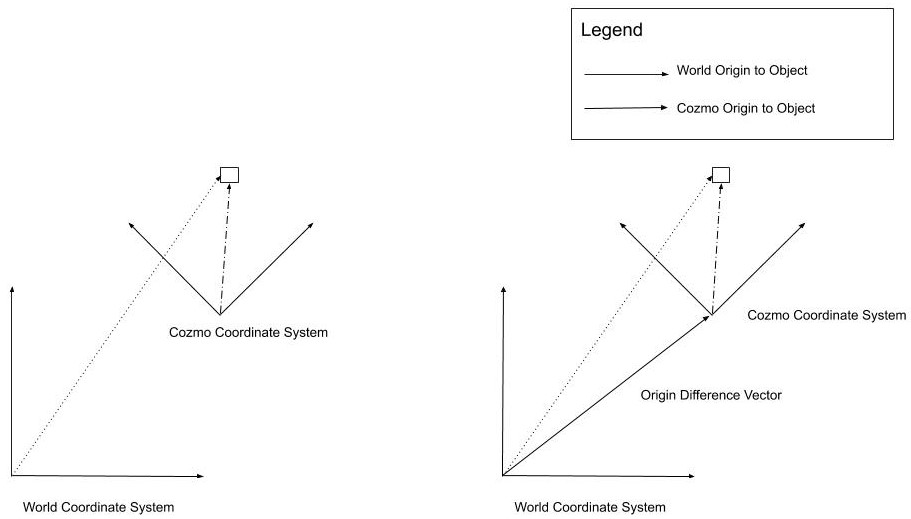
\includegraphics[width=\linewidth]{origin_difference.jpg}
	\caption{The Cozmo origin is not at the same coordinates as the world origin, so a vector in either coordinate system also needs to be translated so that it is relative to the corresponding origin. This can be achieved by keeping track of the Cozmo origin's position relative to the world origin in the origin difference vector $V_d$}
	\label{fig:oridiff}
\end{figure}


The second inconsistency between the two coordinate systems is translation. The Cozmo origin is not at the same coordinates as the world origin, so a vector V also needs to be translated so that it is relative to the corresponding origin. This can be achieved by keeping track of the Cozmo origin's position relative to the world origin in the origin difference vector $V_d$. Figure \ref{fig:oridiff} demonstrates the need for origin difference vector $V_d$ to convert between the two coordinate systems' origins. To find the origin difference vector $V_d$, vector $V_w$ representing Cozmo's pose relative to the world origin in world coordinates is acquired from the overhead camera localizer, and vector $V_c$ representing Cozmo's pose relative to Cozmo's origin in Cozmo coordinates is collected from the Cozmo robot. Then $V_c$ is multiplied by the change of basis matrix $S_{\mathfrak{C}\rightarrow\mathfrak{W}}$ to find vector $V_o$ representing Cozmo's pose relative to the Cozmo origin in world coordinates (Equation \ref{eq:oc}).
\begin{equation} \label{eq:oc}
	V_o = S_{\mathfrak{C}\rightarrow\mathfrak{W}} \cdot V_c
\end{equation}
Finally, the position of Cozmo's origin in world coordinates, the origin difference vector $V_d$, can be calculated by subtracting vector $V_o$ representing Cozmo's pose relative to Cozmo's origin in world coordinates from vector $V_w$ representing Cozmo's pose relative to the world's origin in world coordinates (see Figure 33)  (Equation \ref{eq:do}). 
\begin{equation} \label{eq:do}
	V_d = V_w - V_o
\end{equation}

\begin{figure}[h!]
	\centering
	\begin{subfigure}[b]{0.5\linewidth}
		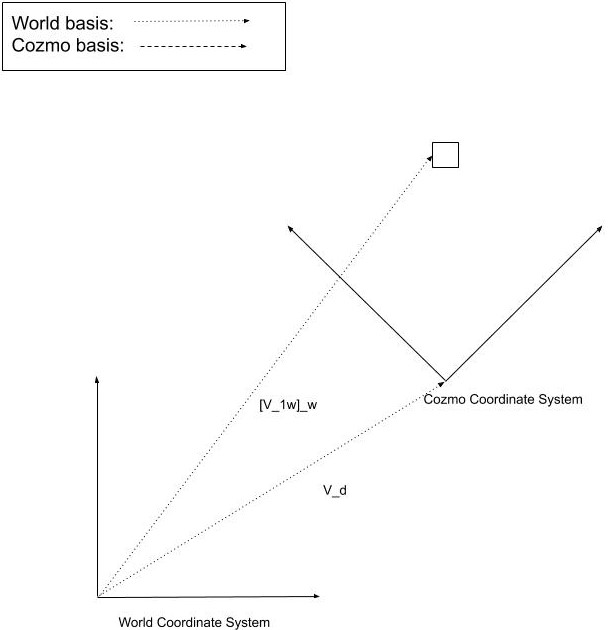
\includegraphics[width=\linewidth]{wc1.jpg}
		\caption{Initial setup}
	\end{subfigure}
	\begin{subfigure}[b]{0.5\linewidth}
		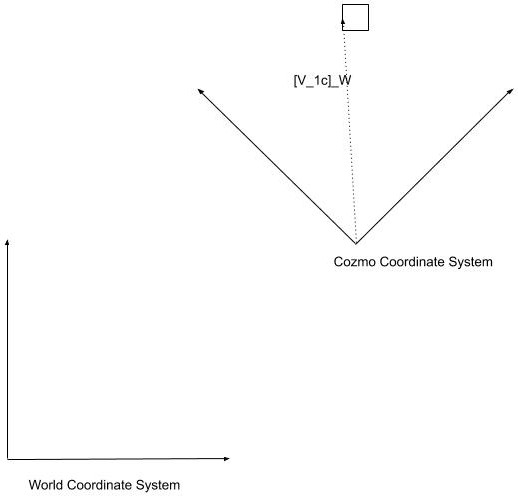
\includegraphics[width=\linewidth]{wc2.jpg}
		\caption{After subtracting origin difference vector}
	\end{subfigure}
	\begin{subfigure}[b]{0.5\linewidth}
		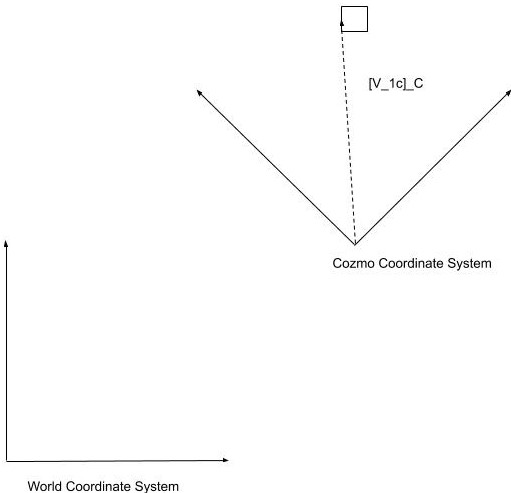
\includegraphics[width=\linewidth]{wc3.jpg}
		\caption{After multiplying by the change of basis matrix}
	\end{subfigure}
	\caption{Changing from world to Cozmo coordinates}
	\label{fig:wtoc}
\end{figure}

The change of basis matrices and the origin difference vector are used to transform to and from the two coordinate systems. To change a given vector $[V_{1w}]_\mathfrak{W}$ in world coordinates to $[V_{1c}]_\mathfrak{C}$ in Cozmo coordinates, first subtract $V_d$, the origin difference vector, so that the vector is relative to Cozmo's origin (Equation \ref{eq:v1c}). This whole process is visualized in Figure \ref{fig:wtoc}
\begin{equation} \label{eq:v1c}
	[V_{1c}]_\mathfrak{W} =  [V_{1w}]_\mathfrak{W} - V_d
\end{equation}
Then multiply the vector $[V_{1c}]_\mathfrak{W}$ by the change of basis matrix $S_{\mathfrak{W}\rightarrow\mathfrak{C}}$, finishing the conversion (Equation \ref{eq:v1c}).
\begin{equation} \label{eq:v1c}
	[V_{1c}]_\mathfrak{C} =  S_{\mathfrak{W}\rightarrow\mathfrak{C}} \cdot [V_{1c}]_\mathfrak{W}
\end{equation}
Our program will return the given object position $[V_{1c}]_\mathfrak{C}$ and rotation $\theta_c$ in Cozmo coordinates.

\begin{figure}[h!]
	\centering
	\begin{subfigure}[b]{0.5\linewidth}
		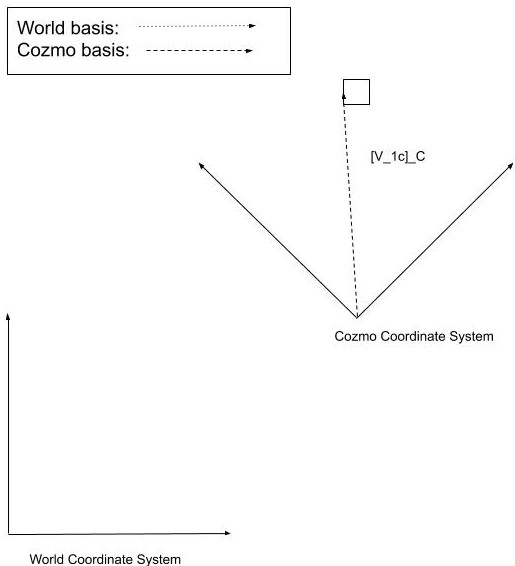
\includegraphics[width=\linewidth]{cw1.jpg}
		\caption{Initial setup}
	\end{subfigure}
	\begin{subfigure}[b]{0.5\linewidth}
		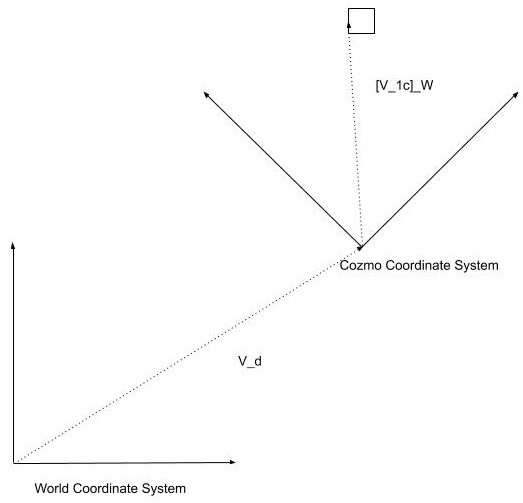
\includegraphics[width=\linewidth]{cw2.jpg}
		\caption{After multiplying by the change of basis matrix}
	\end{subfigure}
	\begin{subfigure}[b]{0.5\linewidth}
		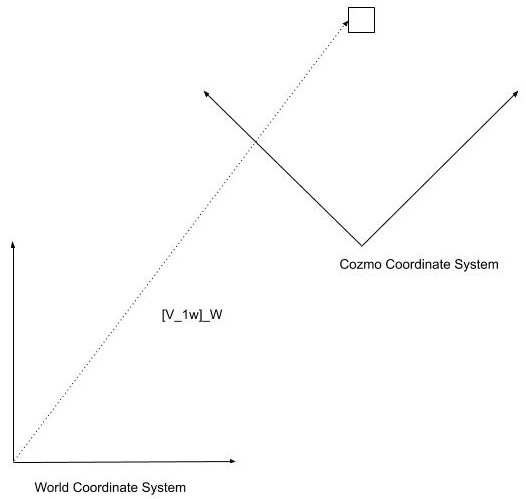
\includegraphics[width=\linewidth]{cw3.jpg}
		\caption{After subtracting origin difference vector}
	\end{subfigure}
	\caption{Changing from Cozmo to world coordinates}
	\label{fig:ctow}
\end{figure}

Conversely as visualized in Figure \ref{fig:ctow}, when changing an arbitrary vector $[V_{2c}]_\mathfrak{C}$ in Cozmo coordinates to $[V_{2w}]_\mathfrak{W}$ in world coordinates, first multiply $[V_{2c}]_\mathfrak{C}$ by the change of basis matrix $S_{\mathfrak{C}\rightarrow\mathfrak{W}}$ (Equation \ref{eq:v2c}).
\begin{equation} \label{eq:v2c}
	[V_{2c}]_\mathfrak{W} = S_{\mathfrak{C}\rightarrow\mathfrak{W}} \cdot [V_{2c}]_\mathfrak{C}
\end{equation}
The vector $[V_{2w}]_\mathfrak{W}$, representing the object pose relative to world origin in world coordinates, is then calculated by adding the origin difference vector, $V_d$ (Equation \ref{eq:v2w}).
\begin{equation} \label{eq:v2w}
	[V_{2w}]_\mathfrak{W} = [V_{2c}]_\mathfrak{W}+ V_d
\end{equation}
In this case, our program will also return the given object position $[V_{2w}]_\mathfrak{W}$ and rotation $\theta_w$ in world coordinates.

\subsection{Update Robot Pose}
Our code encapsulates the said functionality in a Camera Localizer class in Python. To not slow down the overall Soar and Cozmo program, the Camera Localizer spun a separate thread. The update transformation and conversion functions are periodically called in CozmoSoar to recalibrate the robot pose. Because the camera localizer is in a global coordinate frame, and does not rely on Cozmo odometry, the system is free from the cumulative odometry error. It then allows for CozmoSoar to conduct experiments and learn new tasks in an environment without having to account for drift.

\section{Experiment}
To test the efficacy of our apparatus, we devised an experiment of CozmoSoar running with and without the overhead camera localizer. In each experiment setting, a Cozmo robot needs to travel through a corridor and a gateway constructed by bricks marked with fiducials. On the other end of the corridor is a cube that Cozmo needs to pick up. Upon picking up the cube, Cozmo will then turn in place two and a half rotations. At the end of the rotation, theoretically, Cozmo should be facing towards its starting position or the Cozmo origin. Finally, Cozmo needs to turn to the proper rotation and travel back to its starting point without running into the gateway or hitting the corridor walls.

\section{Results}


\section{Discussion}


\bibliography{bib}

\end{document}